\documentclass{beamer}

%-----------------------
%% This template is based on a template developed by the SMCS
%% (Statistical Methodology and Computing Service) at UCLouvain

%-----------------------
% pour faire les slides papiers :
% \documentclass[handout, compress]{beamer}
% \usepackage{pgfpages}
% % 4 par page
% \pgfpagesuselayout{4 on 1}[a4paper,border shrink=5mm, landscape]
% % 2 par page
% \pgfpagesuselayout{2 on 1}[a4paper,border shrink=5mm]

\usetheme{UCL2018}

\usepackage[utf8]{inputenc}
\usepackage[T1]{fontenc}
\usepackage{lmodern}
\usepackage{xspace}
\usepackage{float}
\usepackage{graphicx}
\usepackage{amssymb}
\usepackage{hyperref}
\usepackage{ragged2e}

%% For slides in French
%% \usepackage[french]{babel}
%% \usepackage[cyr]{aeguill}

\usepackage{lipsum}

\theoremstyle{example}
\newtheorem{examplef}{Example}
\newtheorem{examplesf}{Examples}
\newcommand{\ei}{\end{itemize}}

\usepackage{xmpincl}


\title{Probabilistic mapping  of the sub-cellular proteome}
\author[\url{http://lgatto.github.io/about}]{Laurent Gatto}
\date{\today}
\institute[]{CBIO, de Duve Institute, UCLouvain}


\begin{document}

\pdfinfo {/Author(Laurent Gatto - UCLouvain)}


%-----------------------------------------------
% Title page
%-----------------------------------------------

\begin{frame}[plain]
\titlepage
\end{frame}


\begin{frame}%[noframenumbering]
%\thispagestyle{empty}

% Logo UCL a gauche
%% \begin{tikzpicture}
%%   \useasboundingbox (0,0) rectangle(\the\paperwidth,1);
%%   \node[inner sep=0pt] at (1.7,.5) {
\includegraphics[width=.33\textwidth]{UCL_2018}};
%%  \end{tikzpicture}

\justify

{\small \textbf{Abstract:} In biology, localisation is function -
  understanding the sub-cellular localisation of proteins is paramount
  to comprehend the context and full extend of their
  functions. Shotgun mass spectrometry-based spatial proteomics method
  are orthogonal to widely used targeted microscopy-based assay. In
  conjunction with contemporary machine learning, the former enable to
  build proteome-wide protein localisation maps, informing us on the
  location of thousands of proteins. When studying these proteome-wide
  spatial maps, one can learn that while some proteins can be found in
  a single location within a cell, up to half of the proteins may
  reside in multiple locations, can dynamically re-localise, or reside
  within an unknown functional compartment, leading to considerable
  uncertainty in associating proteins to their sub-cellular
  location. Recent Bayesian modelling approaches enable us to mine
  these data, and in particular the dynamic fraction of the spatial
  proteome, in much greater depth. We are now in a position to (1)
  probabilistically model protein localisation as well as quantify the
  uncertainty in the location assignments, and (2) compute a
  probability for, and quantify uncertainty in, whether a protein is
  differentially localised upon cellular perturbation. These
  computational approaches lead to better and more trustworthy
  biological interpretation of these rich spatial proteomics data.  }


\end{frame}


\begin{frame}{Acknowledgements}

  \begin{itemize}

  \item \textcolor{SMCSblue}{Mr Oliver Crook}

  \item \textcolor{SMCSblue}{Dr Lisa Breckels}

  \end{itemize}


\end{frame}


%-----------------------------------------------
% Table of content
%-----------------------------------------------

\AtBeginSection[]{
  \setbeamercolor{background canvas}{bg=UCLblue2}
  \setbeamercolor{section in toc}{fg=UCLblue}
  \setbeamercolor{subsection in toc}{fg=UCLblue}
  \setbeamerfont{section in toc}{size=\large}

  \mode<handout>{
    \setbeamercolor{background canvas}{bg=white}
    \setbeamercolor{section in toc}{fg=UCLblue}
    \setbeamercolor{subsection in toc}{fg=UCLblue}
  }

  \begin{frame}[plain]
    \frametitle{Outline}
    \tableofcontents[currentsection,hideothersubsections]
  \end{frame}

  \setbeamercolor{background canvas}{bg=white}
}


%-----------------------------------------------
% Content
%-----------------------------------------------

\section{Spatial proteomics}


\begin{frame}{Cell organisation - \textbf{localisation is function}}
  \begin{center}
    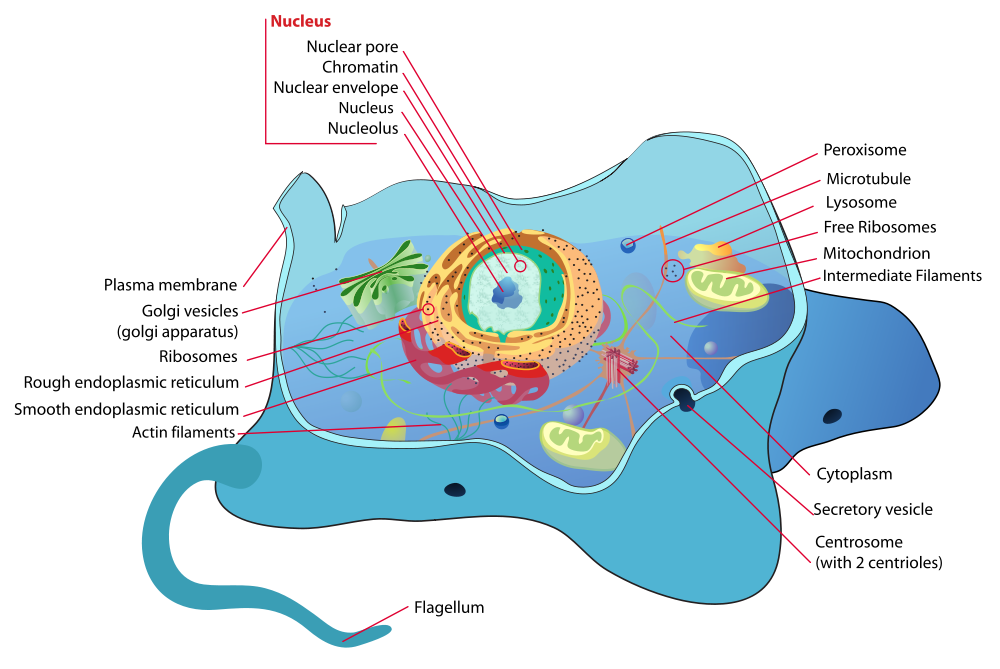
\includegraphics[width=.9\linewidth]{figs/Animal_cell_structure.png} \\
    \textbf{\textcolor{Blue}{Spatial proteomics}} is the systematic
    study of protein localisations.
  \end{center}

  \begin{center}
    \textbf{Localisation -- re-localisation -- mis-localisation}
  \end{center}
  
  \tiny Image from Wikipedia
  \url{http://en.wikipedia.org/wiki/Cell_(biology)}.  
\end{frame}



%-----------------------------------------------
% New section
%-----------------------------------------------

\section{Visualisation}


\begin{frame}{Visualisation}

\end{frame}

%-----------------------------------------------
% New section
%-----------------------------------------------

\section{Computational challenges}


\begin{frame}{Computational challenges}

\end{frame}


%-----------------------------------------------
% New section
%-----------------------------------------------

\section{Novelty detection}


\begin{frame}{Novelty detection}

\end{frame}


%-----------------------------------------------
% New section
%-----------------------------------------------

\section{Quantifying uncertainty}


\begin{frame}{Quantifying uncertainty}

\end{frame}


%-----------------------------------------------
% New section
%-----------------------------------------------

\section{Spatial dynamics}


\begin{frame}{Spatial dynamics}

\end{frame}


%-----------------------------------------------
% New section
%-----------------------------------------------

\section{Behind the scences}


\begin{frame}{Behind the scences}

\end{frame}




%-----------------------------------------------
% Final slide
%-----------------------------------------------

\begin{frame}%[noframenumbering]
%\thispagestyle{empty}

% Logo UCL a gauche
\begin{tikzpicture}
  \useasboundingbox (0,0) rectangle(\the\paperwidth,1);
  \node[inner sep=0pt] at (1.7,2) {
\includegraphics[width=.33\textwidth]{UCL_2018}};
 \end{tikzpicture}
\vspace{.1cm}



\begin{center}
  \textbf{Thank you for your attention}
\end{center}


\bigskip

Contact:

\begin{center}
  laurent.gatto@uclouvain.be – \url{lgatto.github.io/about}
\end{center}
 
\end{frame}


\end{document}
